%%%%%%%%%%%%%%%%%%%%%%%%%%%%%%%%%%%%%%%%%%%%%%%%%%%%%%%%%%%%%%%%%%%%%%%%%%%%%%%%%%%%%
% Template revision history:
% BS2021: Revised by Filip Jorissen, filip.jorissen@kuleuven.be
% BS2019: Revised by Alessandro Prada, alessandro.prada@unitn.it
% BS2017: Initial version by Michael Wetter, mwetter@lbl.gov
%%%%%%%%%%%%%%%%%%%%%%%%%%%%%%%%%%%%%%%%%%%%%%%%%%%%%%%%%%%%%%%%%%%%%%%%%%%%%%%%%%%%%

\documentclass[twocolumn, a4paper,10pt]{article}
\usepackage[top=2.5cm, bottom=2.5cm, left=2.0cm, right=2.0cm,
columnsep=0.8cm]{geometry}
\usepackage{enumitem}
\usepackage[hidelinks]{hyperref}
\usepackage{boxedminipage}
\usepackage{nopageno}
\usepackage{graphicx}
\usepackage{natbib}
\usepackage[font=it]{caption}
\usepackage[usenames,dvipsnames]{xcolor}
\usepackage{listings}
\usepackage{caption}
\usepackage{subcaption}
\usepackage{tabularx}
%-----------------------------SET SKIP SPACES -------------------------------------------------------------------
\setlength{\abovecaptionskip}{0pt}
\setlength{\belowcaptionskip}{3pt}
\setlength{\parindent}{0pt}
\setlength{\parskip}{3pt}
%\renewcommand{\baselinestretch}{0.7}
% FOR enumerates
\setlist{itemsep=-0.1cm,topsep=0.1cm,labelsep=0.3cm}
\setenumerate{leftmargin=*}
\setcounter{secnumdepth}{-1}
%-----------------------------SET FONTS -------------------------------------------------------------------
% Set fonts for title, section and subsection headings
\makeatletter
\renewcommand\title[1]{\gdef\@title{\fontsize{12pt}{2pt}\bfseries{#1}}}
\makeatletter
\renewcommand\section{\@startsection{section}{1}{\z@}{3pt}{3pt}{\normalfont\large\bfseries}}
% \normalfont\large
\makeatletter
\renewcommand\subsection{\@startsection{subsection}{1}{\z@}{\z@}{\z@}{\normalfont\normalsize\bfseries}}
\makeatletter
\renewcommand\subsection{\@startsection{subsection}{1}{\z@}{\z@}{0.1pt}{\normalfont\normalsize\bfseries}}
\renewcommand\refname{References}
%END OF THE SETUP
%%%%%%%%%%%%%%%%%%%%%%%%%%%%%%%%%%%%%%%%%%%%%%%%%%%%%%%%%%%%
% Simulation and visualisation of mitigation and adaption strategy pathways for urban districts
%%%%%%%%%%%%%%%%%%%%%%%%   TITLE   %%%%%%%%%%%%%%%%%%%%%%%%%%%%%%%
%%% Please keep the \vspace{4pt} at the top
\title{%
Simulation and visualization framework for decision making of climate mitigation  																								% Line 1
%%% Please keep the \vspace{4pt} between lines in the title
\vspace{4pt}
and adaptation strategies in new and existing urban development} 																																% Line 2 
%If there is no second line then just put \phantom{Line 2} here
%%% Change or delete text before "\\" on the lines below to keep the layout but don't remove the "\\"
%%% Do not exceed more than 6 lines for authors and affiliations
\author{																																														% Line 3
% Justin McCarty$^1$, Adam Rysanek$^1$
\\ 																				% Line 4
% $^1$The University of British Columbia, Vancouver, Canada
\\ 																																                                                            	% Line 5
% $^2$Institution 2, City 2, Country 2
\\ 																																                                                                % Line 6
% comment the lines below and add \phantom{} lines as needed to reach a total of 10 lines
% \textit{(The names and affiliations SHOULD NOT be included in the draft submitted for review)}
\\ 			 			  	                                                    % Line 7
% \textit{(leave blank up to line 10 - remove line numbering from final version)}
\\ 														                    	% Line 8
\phantom{Line 9}} 																																								            	% Line 9
\date{\vspace{-0.5cm}}	% remove default date and replace the Blank 10th line														                                                            % Line 10
%END OF THE TITLE
%%%%%%%%%%%%%%%%%%%%%%%%%%%%%%%%%%%%%%%%%%%%%%%%%%%%%%%%%%%%
\begin{document}

\maketitle

\section*{Abstract}	% Section headings need to be upper and lower case.
\addtocounter{section}{1}
At present mitigation and adaptations strategies compete for constrained resources within a future of uncertain climate impacts. Meeting decarbonisation goals while implementing robust and resilient adaptation strategies requires an analysis structure that can account for uncertainty as well as depict how the intermingling of strategies may hinder or benefit the ultimate trajectory of actions. The marginal abatement cost curve (MACC) is an indispensable tool for planning mitigation pathways, but has historically not relied upon robust experimental analysis making it notional at best nor has it included a view of adaptation pathways. This study utilizes a newly developed and nearly finished medium-density community in Vancouver, British Columbia, Canada of 15,000 residents as a case study for developing a pathway based MACC. Multiple mitigation and adaptation measures are modeled individually and through exhaustive combination to test their sensitivity on marginal abatement cost and residual cost of climate change. Several visualizations are created to demonstrate several ways of analyzing the resulting large set of data.   

\section*{Key Innovations}
\begin{itemize}
\item Visualization of marginal abatement cost of urban scale building and energy system interventions.
\item Intermingling of climate change mitigation and adaptation strategies in a decision making framework for development planning.
\item The inclusion of embodied carbon as a metric in determining carbon emissions and marginal abatement cost.
\item Contribution of an open-dataset of simulated demand, cost, and emissions for use in reanalysis and further studies.
\end{itemize}

\section*{Practical Implications}
Open-source simulation tools can be used to test the sensitivity of different decarbonisation and adaptation strategies for an urban area, allowing planners better models to make well-informed planning decisions. The resulting visualizations of this study offer a sample of this, as well as an example of a comprehensive urban building energy model. The results also raise questions about decarbonization pathways in British Columbia after strategies such as fuel switching are implemented, reducing the majority of emissions, but not entirely creating zero-carbon communities. 

%---------------------------------------------------------------------------------------
\section*{Introduction}

Atmospheric concentrations of carbon dioxide are just over 410 parts per million, while recent estimates from the \citet{noauthor_state_2020} situate the Northern Hemisphere’s land and ocean surface temperature anomaly at 1.29°C from baseline (1961-1990). This may not be considered a consistent level of \textit{global warming}, but it does indicate a the dangerous warming trend facing human and non-human systems. Climate change impacts are now being recognized as burdens on economic and social systems \citep{frame_climate_2020}. Implementing adaptation strategies within the built environment is necessary to increase social resilience, protect safety and life, and prevent economic damage with the potential to bolster all of the above \citep{schunemann_mitigation_2020}. Simultaneously, the mitigation of present emissions, the abatement of possible future emissions, and the sequestration of atmospheric carbon is necessary to curtail increasingly dangerous and catastrophic levels of warming. This process of carbon drawdown is very familiar within studies of the built environment with strategies posed for transportation, buildings, agriculture, forestry, and other landuses. Mitigation and adaptation strategies though are rarely evaluated simultaneously in the context of urban development.

In the presence of limited resources and a range of objectives, the cost and benefit of proposed strategies need to be assessed on their own and while interacting with other strategies, as well as under the uncertainty of climate change and human action. The interaction of strategies is a key factor explored in \citet{rysanek_using_2013}, where exhaustive simulation is applied in the modeling of fifteen individual building retrofit strategies (a total of 32,768 unique combinations). From this, a database of simulated retrofits specific pathways for a single building can be generated. However, \citet{rysanek_using_2013} note that this process may not be desirable for every retrofit project that concerns only one building as the overhead cost of developing such a model is large and requires extensive computing resources. However, in the application of urban retrofit modeling for the purposes of enhancing policy making and incentive creation this framework could prove useful.

Introducing the scale of a neighborhood or even entire city affords the use of an extensive modelling framework as described above, but further uncertainty is encountered in this problem space when considering urban development. No longer is the model concerned with answering a single question about a single existing building - how do we mitigate the most carbon at the lowest price? Now, the model is being applied in the context of an existing area where buildings and empty plots face a \textit{known-unknown} trajectory of new development, redevelopment, and no change. This brings in the concept of a development timeline during which differing scales of development may occur.

The resulting simulation database can be used to assess decarbonization pathways that align with development trajectories and/or different degrees of global warming. The difficulty though is in interpreting a large quantity of simulation data for its salience in the mitigation and adaptation planning space. Several have proposed marginal abatement cost curves (MACCs) as a useful metric to compare strategies, while \citet{kesicki_marginal_2012} points out that their use should be tempered with caution related to the lack of interaction of strategies in typical MACCs, a point taken up in \citet{rysanek_using_2013} through an underlying sequential and exhaustive simulation framework \citep{afshari_life-cycle_2014,ibrahim_methodology_2016}. Applying this same framework to the task of determining optimal decarbonization pathways through mitigation strategies can result in a viable set of MACCs for planing and policy support.

The literature on MACCs has not yet involved adaptation strategies as a form of emissions mitigation. However, as noted earlier adaptation and mitigation strategies, may be decided upon from the same funding perspective and therefore need to be considered together. Therefore this study integrates several adaptations strategies into the simulation process. These adaptation strategies are evaluated on the basis of marginal abatement cost, as well as their influence on adaptation within the development. Therefore, mitigation strategies are equally evaluated as adaptations strategies. 

This study will test the performance of eight strategies alongside one development pathway and two climate change pathways, simulated at two points in time (2050 and 2080), for a case study community in southwestern Canada; Wesbrook Village, Vancouver, British Columbia (BC). A baseline urban building energy model (UBEM) was created to represent the development of the community to-date, shown in Figure \ref{fig:wesbrook_base} alongside the future development and climate change pathways.

% \begin{figure}
%     \centering
%     
\includegraphics[scale=1.5]{figures/sample_sequence.eps}
%     \caption{Each scenario iterated through 256 combinations of strategy implementation.}
%     \label{fig:sample_sequence}
% \end{figure}

% \begin{figure}
%     \centering
%     \includegraphics{}
%     \caption{The baseline UBEM for Wesbrook Village in BC.}
%     \label{fig:wesbrook_base}
% \end{figure}

\subsection*{Wesbrook Village} 
Simulation will be exhaustive of the different combinations in the pool of strategies and scenarios allowing each strategy to be measured independently as well as determine combinations that are more or less efficient than individual implementation under the entire range of uncertainty, diagrammed in Figure \ref{fig:sample_sequence}.

Wesbrook Village and the neighbouring Stadium Road are new communities that expected to reach 715,925 sqm. of residential floor space and 10,000 sqm. of non-residential floor space by 2040. It is the part of a larger community plan led by the development arm of The University of British Columbia (UBC) \citep{ubc_planning_ubc_2020_SR, ubc_planning_ubc_2020_wb}. The baseline for this study is taken at the end of 2020, where the development has completed its fifteenth year. The development, referred to throughout the study as \textit{Wesbrook}, is a compelling case study as it can be considered a model of medium-density new development for BC and North America at large. Building code for the community is modeled after the aspirational provincial code made more strict through a continuous review with the most recent version taking effect in January 2021 and targeting net-zero energy ready (NZER) by 2032; NZER buildings are built such that with the addition of solar panels or renewable technologies they would consume only as much energy as they produce. The energy system is a mixture of grid-connected systems, in building natural gas boilers, and a district heating system that supplies hydronic baseboard and floor heating systems as well as domestic hot water. This district heating system, described in the context of a UBEM in \citet{mccarty_accepted_2020}, is designed to switch from natural gas boilers to heat pumps amplified by waste heat from a nearby particle accelerator facility but still with peaking boilers fueled by natural gas. Cooling services have yet to considered in spec-residential development in BC as the climate has historically allowed comfort to be achieved in the peak of summer through natural ventilation; research however indicates that this may become an obsolete design standard due to climate change \citep{rysanek_forecasting_2021}. The intention with the code development for this community is that cooling will be required within a decade \citep{noauthor_residential_2021}.

\subsubsection*{Retrofit and New Development Trajectory}
The majority of Wesbrook has been completed as of 2020, with 50\% of the total expected build-out of 725,925 sqm. remaining between now and the mid-21st century. As indicated in Figure \ref{fig:wesbrook_base} the yet-to-be-completed development will be assessed in the model through the future periods. While in less centrally planned and developed communities tackling development uncertainty would require a more thorough economic model, the Wesbrook planning and development scheme is well laid out in master-planning documents \citep{ubc_planning_ubc_2020_wb}. The simulation framework is built from a baseline in 2020 of the completed development up to 2020. Two more time periods were simulated, the first in 2050 and then in 2080. The base-case for each time period assumes that the stock of buildings that were simulated in the previous time-step (existing) were retrofitted with similarly performing technologies and components. New buildings are however built to a performance profile modeled after the changes in the municipalities building performance code (\citep{noauthor_residential_2021}). While it is expected that the future will hold more advanced technologies, code development is capped at the introduction of the NZER requirements.

% \begin{table*}[h]
%     \vspace{-5pt}   % Please use appropriate negative vspace to remove the space above/belovw the Table
%     \caption{The first two-column table.}
%     \label{tab:code_trajectory}
%     \centering
%     \begin{tabular}{ | c | c | c | }
%         \hline
%         \bf{Year} & \bf{Code Name} 2 & \bf{Performance Note} \\
%         \hline
%         2005 & REAP2.1 & Wall U-Value = 0.4 W/m²K \\
%         \hline
%         2005 & REAP2.1 & Wall U-Value = 0.4 W/m²K \\
%         \hline
%         2005 & REAP2.1 & Wall U-Value = 0.4 W/m²K \\
%         \hline
%         2005 & REAP2.1 & Wall U-Value = 0.4 W/m²K \\
%         \hline
%     \end{tabular}
%     \vspace{-5pt}   % Please use appropriate negative vspace to remove the space above/belovw the Table
% \end{table*}

\subsection*{Mitigation and adaptation decision tools}
\citet{rysanek_using_2013} expanded on the use of marginal abatement cost curves as a tool for planning retrofit pathways in single building optimization. The authors commentary was that by failing to consider technical and economic interactions MACCs such as those proposed by \citet{mckinsey__co_climate_2010} were more \textit{illustrative} than planning tools. Without accounting for the additionality of measures many MACCs fall into this grouping and limit their overall effectiveness. \citet{kesicki_marginal_2012} acknowledges temporal interactions as an additional dimension that need to be considered when constructing MACCs. Traditionally MACCs were developed for annual-planning and more recently, as ambition has grown, so too have their temporal scales. These interactions can be summarized as understanding how investments made in the past may affect the outcome of the MACC, similar to the issue of technical and economic interactions. In planning buildings or infrastructure with MACCs this becomes a significant feature to consider as selecting investments to implement, one typically does so along an investment pathway. 

It is also of particular importance when developing infrastructure or buildings to consider the impact of a changing climate. Adaptation is prevalent in designing buildings in proximity to rising seas, with strategies ranging from hard measures such as levies and dams to soft measures such as wetland restoration \citep{pachauri_climate_2015}. Evidence is pointing to the need to consider other impacts, such as overheating risk due to generally warmer days, nights with less cooling capacity, and more intense heat waves \citep{lomas_overheating_2017,rysanek_forecasting_2021}. Measuring adaptation is a contentious field, as what defines successful adaptation is not as simple to calculate as net carbon emissions \citep{pachauri_climate_2015}. \citet{brooks_tracking_2011} suggests several general criteria by which successful adaptation can be assessed: feasibility, efficacy/effectiveness, efficiency, acceptability/legitimacy, equity, and sustainability. The same authors also discuss the concept of \textit{Maladaptation}, or the inadvertent increase in vulnerability to climate change as a result of development, which has equal importance to adaptation planning of buildings. For all criteria though, measures begin with assessing vulnerability of a subject to a stressor or collection of stressors. In the case of coastal development, a building's adaptive capacity and success can be measured by its vulnerability to increasingly intense sea level rise and storm surge. In the case of this study the stressor is heat gain and the vulnerability of a building to overheating. 

%---------------------------------------------------------------------------------------
\section*{Methods}

\begin{table*}[ht]
    \vspace{-5pt}   % Please use appropriate negative vspace to remove the space above/belovw the Table
    \caption{Each strategy as it was applied in the simulations.}
    \footnotesize
    \label{tab:strategies}
    \centering
    \begin{tabularx}{\textwidth}{|X|X|X|}
        \hline
        \bf{Strategy} & \bf{Description} & \bf{Scale} \\
        \hline
        Adjust Comfort Threshold & Raise cooling setpoints 1C and reduce heating setpoints 1C & All Buildings \\
        \hline
        Green Roof & Install green roofs for insulative, albedo, and heat gain benefits. & All Buildings \\
        \hline
        Deep Envelope and HVAC Retrofit & Install heat pumps for space heating and DHW along with high performance shells and reduced window-wall ratios & Existing Buildings \\
        \hline
        Passive House & Require passive house building codes for envelope. & New Buildings \\
        \hline
        Heat Pumps & Install heat pumps for space heating, cooling and DHW. & All buildings \\
        \hline
        Mass Timber & Construction must utilize mass timber. & New Buildings \\
        \hline
        Seawater Cooling Loop & Buildings get space cooling from heat pump that is amplified with a seawater cooling loop & All Buildings \\
        \hline
        Rooftop Photovoltaic & Install grid-tied rooftop solar with net-metering & All Buildings \\
        \hline
    \end{tabularx}
    \vspace{-5pt}   % Please use appropriate negative vspace to remove the space above/belovw the Table
\end{table*}

\subsection*{Urban Building Energy Model}
The simulation framework utilizes an extension of the City Energy Analyst (CEA) demand forecasting model \citep{fonseca_integrated_2015,fonseca_city_2016,the_cea_team_city_2020}. The CEA enables simulations of urban and neighborhood scale energy systems, as well as independently operating buildings. It is a hybrid dynamic statistical model that allows for efficient processing times, a necessity for large simulation sets such as the one in this study. These urban building energy models (UBEM) are low-level of detail geometrically described by their heights above and below ground, window to wall ratio, and composition of envelope, HVAC, and energy supply traits. 

The UBEMs consists of a base-case of development and two future states of development, one in 2050 and another in 2080. The base-case was simulated once to tune the model. Each of the future states of development were simulated once for each combination of strategies under both climate change scenarios for a total of 1024 simulations.  

\subsection*{Boundary conditions}
The EnergyPlus Weather (EPW) file for Vancouver, BC produced by \citet{cwec_2016} was morphed, following the algorithms set out by \citet{belcher_constructing_2005} and expanded upon by \citet{jentsch_climate_2008}. For a variable such as temperature being morphed, the monthly delta of a region's historical climate models and a future climate model is calculated to apply to one of several morphing algorithms to adjust the hourly values contained in an EPW file. Variations on the morphing process have been found, accounting for different shortcomings or the availability of more resolute climate model data to describe a region's specific topographic or climatic uniqueness that may not be captured in a typical climate model's often 100km x 100km grid.

The morphing process in this study differs from previous examples in that it was able to make use of the latest generation of global climate models \citep{oneill_scenario_2016}. The morphing process took into account an ensemble of 24 models for calculating projected hourly temperature, solar radiation, cloud cover, relative humidity, wind speed, and air pressure. Two climate pathways are followed, discussed in this paper as the \textit{best-case} and \textit{worst-case} scenarios. These are \textit{Shared Socioeconomic Pathway 1} (SSP126) and \textit{Shared Socioeconomic Pathway 5} (SSP585)
defined in \citet{oneill_roads_2017}. The four morphed EPWs are described in Figure \ref{fig:weatherfiles}.

\subsection*{Strategies}
Eight mitigation and adaptation strategies were selected to evaluate under the development pathways and climate change pathways. The strategies, described in Table \ref{tab:strategies}, reflect larger interventions into either existing buildings, new buildings, both, or the underlying energy system in the community. A strategy is implemented alone as well as in combination with the other seven to understand its range of potential impacts, which assists the decision-making framework in determining a pathway to implement strategies.

\subsection*{Simulation}
For each development period and under each climate change pathway the same eight strategies for carbon mitigation and climate change adaptation to a changing climate were evaluated for their marginal cost of carbon abatement across the whole the Wesbrook development. The simulation procedure for each scenario began with the base-case, under which no strategies were implemented, following with 255 iterations where strategies where implemented alone and in combination with each other. This was repeated across both development pathways and both climate change pathways, leading to 1024 iterations of the model. The advantage of the underlying simulation technology, CEA, is that demand forecasting can be performed parallelized through multithreading, greatly improving processing time at three minutes per iteration. At the time of writing radiation analysis was not able to be brought out of a single CPU core and thus steps were taken to minimize the amount of times the command was used as the processing time for the ~120 buildings in the UBEM was 25 minutes. In each scenario only 16 experiments required unique radiation profiles. These were run first in the loop of 256. This is due to some strategies not influencing the radiation simulation output, such as in the \textit{Mass Timber} case. The 240 simulations that followed then copied the appropriate output files from the radiation analysis. District heating primary energy requirement was modeled post-simulation as the system present in Wesbrook Village is nuanced to its efficiency and fuel source over the day. This process is described in the following section on "Operational and embodied carbon". 

A single entire simulation process (1024 iterations) required 64 hours of processing, utilizing 14 threads from an Intel i9-9900 8-core CPU at 4.6GHz, requiring 20GB of free RAM and an end storage requirement over 2TB of uncompressed results files. This detail is mentioned to help readers understand the scale of computing required to undertake simulations of this scale and to seek methods and functions that optimize processing times. 

\subsection*{Total Annualized Cost}
Components and technology costs was gathered through several data sources, \citep{noauthor_cpcn_2014,schlueter_3for2_2016,salasovich_energy_2016,kegel_life_nodate,gordian_rsmeans_2020}. The authors recognize that cost is a highly uncertain data point to incorporate into building models. While the entire capital and operating cost of each building is not encompassed the cost of components and technologies that are affected by strategies are included, making the calculation of net cost between the base-case and an intervention plausible. Cost is assessed as the 30-year total annualized cost (TAC) from within the City Energy Analyst, applying a 5\% discount rate.

\subsection*{Operational and embodied carbon}
Operational carbon is taken as the carbon emitted over a 30 year period from each building as a result of energy consumption for plug-load, heating and cooling, and ventilation service. BC's electrical grid is served by a hydroelectric power provider and is a low-carbon source, at 10.8 kgCO2e/kWh \citep{bc_ministry_of_envrionmetn_and_climate_change_strategy_bc_2019}. The district heating provider intends for the system to fed entirely from natural gas boilers until 2023 at which point the transition to a more complex system of natural gas peaking boilers and waste heat fed heat pumps will be created. This system was previously modelled in \citet{mccarty_accepted_2020}. Its carbon intensity was estimated to be between an annual average of 10.8 and 180.0 kgCO2e/kWh. The range is due to fluctuations in the amount of natural gas used in the system, as well as the amount of waste heat available to create a more efficient lift in the heat pumps. Figure \ref{fig:district_heat_explainer} describes a baseline case of performance with the system. Limits imposed on heat pump and waste heat capacity are drawn from the operator in \citet{noauthor_infrastructure_2014}.

The embodied carbon of components and technologies of the models was gathered, similarly to the cost data, from a variety of sources \citep{jones_ice_2019, droguett_embodied_2019,rodriguez_embodied_2019,c-change_labs_embodied_2020}, and are cradle-to-gate accounts of embodied carbon. The limitation with disparate data sources in this portion of the research generally has to do with the geography of the components involved. An effort was made to first gather data from sources specific the BC or the Pacific Northwest region of the US and than from North America as a whole, before seeking data from further away. 

\subsection*{Adaptation and mitigation}
Mitigation was evaluated using the marginal cost of carbon abatement. Marginal abatement cost requires two metrics, the first being the net amount of carbon emitted between a base-case and scenario and the net cost between the base-case and scenario. In this study the base-case is the first iteration of the 256, where no strategies have been applied. Carbon emissions are calculated as the embodied carbon of capital expenditures and the 30-year operating carbon. Cost is the 30-year TAC.

Adaptation was considered as the capacity of a building to remain in its comfort threshold while also mitigating carbon emissions. The threshold is set to setpoints of the buildings, which are in a majority 21C for heating and 26C for cooling - except where changed by the first strategy. The deviation from the threshold is measured as the percent change from the baseline in \textit{total hours outside of the threshold} for each iteration. For instance if in the baseline case \textit{total hours outside of threshold} are 2000 and in an experiment the \textit{total hours outside of threshold} are 1500, we have seen a 25\% decrease. 

%---------------------------------------------------------------------------------------
\section*{Results}
The simulation procedure was executed for 1024 scenarios, producing hourly demand results for each building within the simulation space, as well as annual cost and emissions results for each building. For iterations in which rooftop-photovoltaic was an option a set of results was generated to be used in correcting total grid-demand for the electricity generated by the rooftop-photovoltaic. A final open-database is available in the repository mentioned in the abstract. From these iterations several MACCs were constructed in Figures \ref{fig:MACC_budget}, \ref{fig:MACC_threshold}, \ref{fig:MACC_true_noDH}, and \ref{fig:MACC_true_DH}. These are discussed at more in the following sections but differ in that they are constructed following two logics. The first two are \textit{illustrative} MACCs in that they present a set of possible interventions, but not necessarily a pathway through which those interventions can be connected. The latter two are \textit{true} MACCs in that each bar represents a singular strategy where the MAC considers the economic and technical impacts of the other presented strategies and those that may be included in the strategy set but are not included in the MAC, as they do not abate carbon by themselves, as seen in Figures \ref{fig:MACC_true_noDH_waterfall} and \ref{fig:MACC_true_DH_waterfall}. 


\begin{figure*}
\centering
\begin{minipage}[b]{.45\textwidth}
    \hspace*{-1.05cm}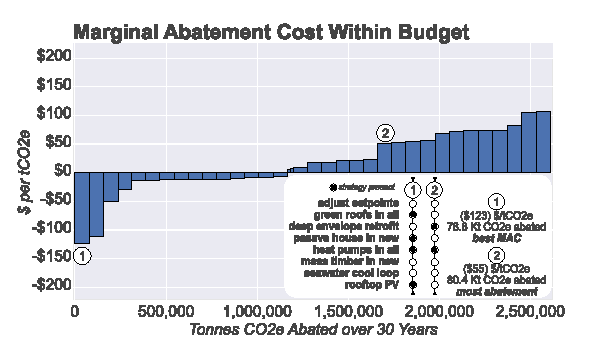
\includegraphics[scale=1.0]{figures/budget_macc.eps}
    \caption{Illustrative MACC made assuming a budget of \$11 million in net cost was permitted for any plotted strategy-set.}
    \label{fig:MACC_budget}
\end{minipage}\qquad
\begin{minipage}[b]{.45\textwidth}
    \hspace*{-.4cm}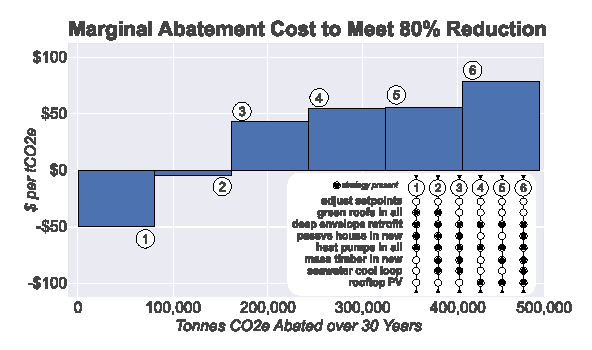
\includegraphics[scale=1.0]{figures/threshold_macc.eps}
    \caption{Illustrative MACC made assuming an emissions reduction threshold of 80\% was necessary for any plotted strategy-set.}
    \label{fig:MACC_threshold}
\end{minipage}
\end{figure*}



\subsection*{General Performance}
Figure \ref{fig:cross_plot} displays net-cost and gross emissions for each iteration within each of the four scenarios. Three groups tend to emerge with the most start difference being that one group is emitting far more than the other two. This is a result of those scenarios still relying on the natural-gas based heating system. This difference is apparent across both climate change pathways, leading to a conslusion that the impacts of more severe climate are not disrupting mitigation efforts in the model. It appears to enable it to an extent. Comparing the highlighted groups of similar scenarios between the best-case and worst-case scenarios a decrease in lifetime emissions is apparent. We suspect that this is due to the warmer temperatures reducing the heating seasons as well as enabling the district to remain below the heat pump capacity more of the year. Figure \ref{fig:comapre_district} shows this in the operation of the district in the baseline cases from each climate scenario.

\begin{figure}[hbt]
    \centering
    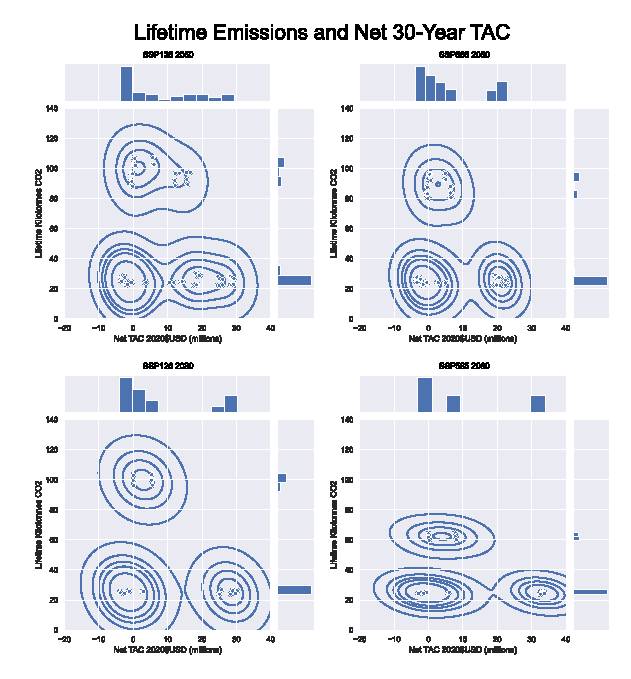
\includegraphics[scale=0.8]{figures/general_results_box.eps}
    \caption{General results from the iterations presented across total emissions over 30 years and net 30-year total annualized cost.}
    \label{fig:cross_plot}
\end{figure}

\subsection*{Visualizing decision making}
Marginal abatement cost and the adaptation metric were plotted to evaluate the Pareto front of each scenario. For each of the four combinations of development and climate change pathway, Figure \ref{fig:pareto_plot} highlights the best performing set of experiments using a convex hull, pareto frontier. The adaptation metric is altered in these plots to show the remaining percentage of \textit{hours outside of the threshold}, where the optimum would be 0\%. The figure as a whole was created under that assumption that only one strategy can be implemented at a time, with the topmost row containing all 255 experiments for each scenario and the following rows one less strategy implemented until the bottom row which contains only a single strategy implemented. This format allows us to view the optimal target and then evaluate how to achieve that by selecting strategy combinations in reverse, as suggested by the overlaid pathway. In several cases no optimum set is reached due their only being one optimum. As a decision-making tool these types of graphs allow us to compare two base-metrics for economic decision making about mitigation and the effectiveness of the strategies as adaptation efforts.

MACCs were drawn as another form of visualising decision making. Figure \ref{fig:MACC_budget} is not a \textit{true} MACC in that you can only implement one of the strategy-sets, represented by the bars. However, it improves on previous \textit{illustrative} MACCs in that the bars do not unnecessarily represent single strategy interventions, but rather a set of strategies. It was drawn to assist in planning under the assumption that planners are expecting a worst-case climate change scenario by the end of the century and have set a budget of an additional \$11,000,000 that could be invested across the development on mitigation and adaptation strategies. The drawn MACC then presents every possible combination under the development and climate change trajectory that falls below the budget, selecting \textit{01011001} at the marginal abatement cost of -\$123. Another \textit{illustrative} MACC was drawn, seen in Figure \ref{fig:MACC_threshold} assuming an emissions reduction threshold of 80\% by 2050 under the best-case climate scenario. All bars represet strategy-sets that would reach that reductions total, ultimately \textit{0111000} is chosen at the marginal abatement cost of -\$50.


\begin{figure}[hbpt]
    \centering
    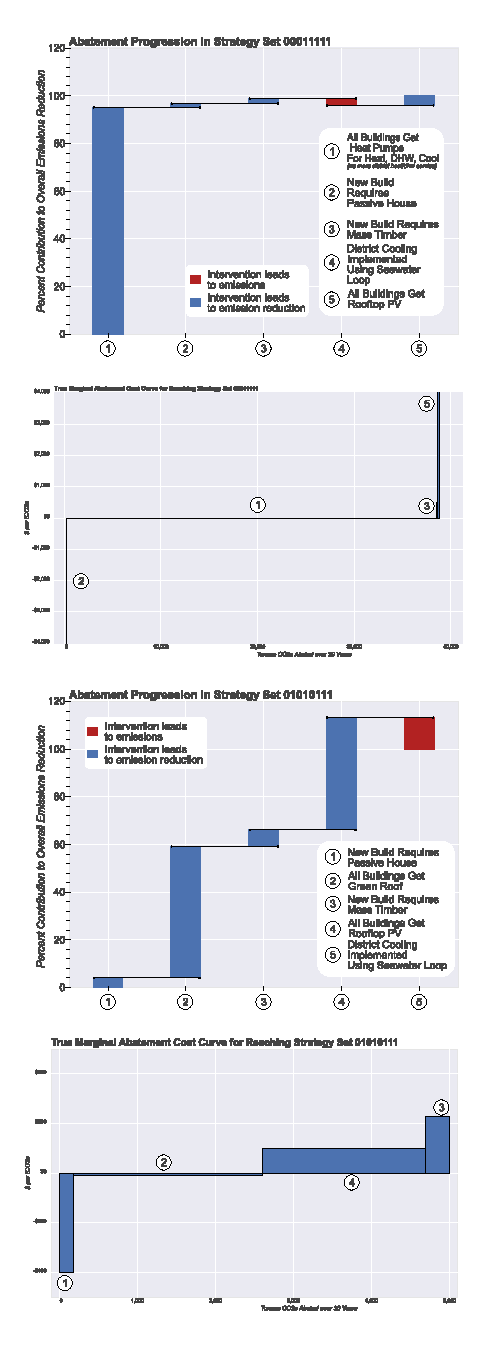
\includegraphics[scale=0.8]{figures/true_maccs_waterfalls_both.eps}
    \caption{Plotting marginal abatement cost and the adaptation metric to serve as a canvas for pathway planning.}
    \label{fig:true_macc_both}
\end{figure}


Of the two \textit{true} MACCs used in this study, the first represents a strategy-set that was chosen based on a high degree of adaptability present, while also abating a large amount of emissions. This was done under the worst-case climate scenario and the selected strategy-set \textit{00011111} is highlighted in Figure \ref{fig:pareto_plot}. Figure \ref{fig:MACC_true_noDH} describes how each strategy contributes to the overall decrease in emissions. The MACC is shown in Figure \ref{fig:MACC_true_noDH} where the first strategy, the installation of heat pumps in all buildings to service space heating and cooling as well as domestic hot water, contributes to the bulk of the emissions reduction. This is due to the impact that moving away from the district heating system, which has the potential to use natural gas if heating and DHW load exceeds the district's heat pump capacity. The majority of the abatement can be attributed to the heat pump strategy, removing natural gas from the fuel mix, while the other strategies can be said to lending to adaptability. This point about the fuel mix will be returned to more in the discussion, but raises that question about how to affordably meet zero-carbon targets after fuel-switching has been achieved. This scenario only achieves 67\% emissions reduction over the baseline by 2080.


% \begin{figure}[t]
%     \centering
%     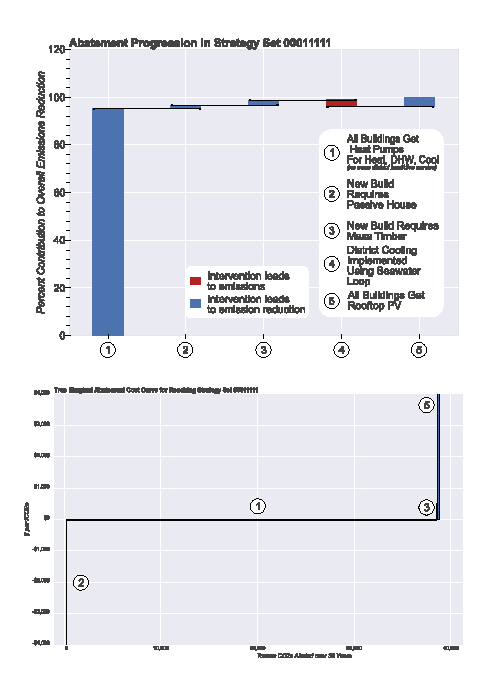
\includegraphics[scale=0.8]{figures/true_macc_noDH_waterfall_comb.eps}
%     \caption{Plotting marginal abatement cost and the adaptation metric to serve as a canvas for pathway planning.}
%     \label{fig:MACC_true_noDH}
% \end{figure}

A second \textit{true} MACC was generated under the plan to abate as many emissions as possible while continuing to use the district heating system, under the worst-case climate scenario. Figure \ref{fig:MACC_true_DH} describes how each measure contributes to overall emissions reduction. The resulting MACC shows a more consistent scale of MAC and overall abatement between measures that the previous example, but total abatement is only 8\% of the baseline's emissions.



% \begin{figure}[t]
%     \centering
%     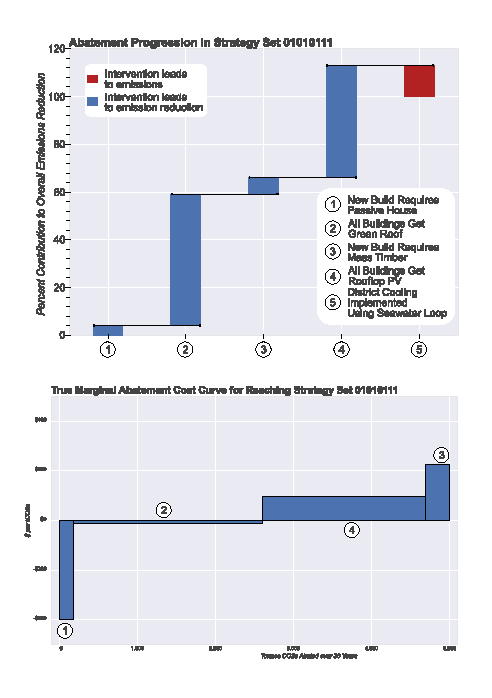
\includegraphics[scale=0.8]{figures/true_macc_DH_waterfall_comb.eps}
%     \caption{Plotting marginal abatement cost and the adaptation metric to serve as a canvas for pathway planning.}
%     \label{fig:MACC_true_DH}
% \end{figure}


\begin{figure*}[hbpt]
    \centering
    \includegraphics[scale=0.8]{figures/optimal_plots.eps}
    \caption{Plotting marginal abatement cost and the adaptation metric to serve as a canvas for pathway planning.}
    \label{fig:pareto_plot}
\end{figure*}

%---------------------------------------------------------------------------------------
\section*{Discussion}
The use of MACCs, \textit{true} and \textit{illustrative}, offers urban scale energy and development planners a way to compare different types of interventions for their merit as adaptation and mitigation interventions. This analysis is robust in that it simulates the technical and financial interaction of the proposed strategies under multiple climate change pathways and following different development trajectories. The first limitation lies in the not-so-explicit temporal interaction of the interventions. Each building was modeled as having its own unique construction and retrofit dates, which contribute to the emissions and total annualized cost profile for each run of the district energy model. While unique in their start and end date they are all set on a 30-year time horizon for all elements replacement. For some building technologies this may be a realistic time horizon for design-life, for many others it is not. Future efforts need to consider equipment and technology replacements more actively while also engaging the temporal simulation steps at more fine scales, possibly ten-years. 


\subsection*{Strategy choice}
A major limitation in the framework underpinning this study is the finite space of strategy choice. We test eight strategies here that are applied generally across the district. This may not always be a problem if prior to the study a strategy evaluation study is conducted or subject-matter experts are brought in to help establish priors. Future efforts need to be more precise with strategy implementation based on building or site need. 

\subsection*{Abatement after fuel-switching}
The context for this study sets up an interesting proposition within BC. The electrical grid is majority hydroelectric. Emissions within the building sector are therefore driven by natural gas use, either on site or within district systems. The two \textit{true} MACC cases show that in order to reach large reductions over the baseline condition the use of natural gas must be eliminated. This however raises the point of how abatement should continua once the significant reductions are made and systems are then relying on a near-carbon free grid. Future building code intends for new buildings to be net-zero \textit{energy} ready, but this study showed in testing rooftop photovoltaic that for this type of density, just rooftop panels are not going to generate significant amounts of energy or contribute to emissions reductions; in the worst-case climate scenario rooftop panels alone reduced emissions by 4.4\%. 

Additionally building-based sequestration methods offer a potential avenue for meeting net-zero \textit{carbon} goals \citep{skullestad_high-rise_2016, zeitz_comparing_2019}. This study did not consider the Mass Timber strategy to be carbon sequestering, but it is less intensive than cement-based building, leading to between 60 and 300 Tonnes of carbon abated, depending on the development scenario.


%---------------------------------------------------------------------------------------
\section*{Conclusion}
In this study the output of 1024 different urban building energy simulations was discussed in the context of use marginal abatement cost curves and complimentary visualizations to make decisions regarding mitigation and adaptation planning for a medium-density community in Vancouver, British Columbia. The simulations were differing combinations of development completeness of the community, climate change pathway (between best- and worst-case scenarios), and eight mitigation and adaptation strategies. 

The resulting MACCs were created from two perspectives. First the \textit{illustrative} MACCs (Figures \ref{fig:MACC_threshold} and \ref{fig:MACC_budget}) provide general guidance on choosing sets of strategies to achieve mitigation under different planning constraints. The \textit{true} MACCs (Figures \ref{fig:MACC_true_DH} and \ref{fig:MACC_true_noDH}) reveal how the individual strategies within a set interact to technically and financially to ultimately abate a certain amount of carbon. The candidate for the one of the \textit{true} MACCs was selected based on a mixture of adaptation and mitigation criteria using a plot of pareto optimums (Figure \ref{fig:pareto_plot}). This enables planners to begin to assess adaptation targets alongside abatement.

The analysis had limitations discussed in the literature on using MACCs for decision-support. These include being more realistic about building technology and component lifetimes, which requires the framework to consider retirement. As well the study is constrained by computational resources and known mitigation and adaptation strategies for the site. Future studies should seek to better understand either through exploratory analysis or expert elicitation, which strategies are reasonable for the market and context. This will also aide in developing a cost and carbon database.

The results of the simulation provide more than an example for decision-support visualization. In comparing the results we see a large difference in abatement between systems that continue to rely on natural gas into the latter half of the century and those that transition to a hydroelectric fed grid. The large jump between the two provokes the thought of how deep emissions reductions will be achieved when demand from space heating, cooling, DHW, and plug load are being met by affordable near-zero carbon electricity.

%---------------------------------------------------------------------------------------
\section*{Acknowledgment}


%---------------------------------------------------------------------------------------
\footnotesize
\bibliographystyle{BS2021}
\bibliography{bs2021_ref}
% \newpage
% \onecolumn
% Please \textbf{do not} include this disclaimer in your paper.  You will be required to accept these conditions when you  submit your paper via the web site.
\end{document}
